
%% bare_conf.tex
%% V1.4b
%% 2015/08/26
%% by Michael Shell
%% See:
%% http://www.michaelshell.org/
%% for current contact information.
%%
%% This is a skeleton file demonstrating the use of IEEEtran.cls
%% (requires IEEEtran.cls version 1.8b or later) with an IEEE
%% conference paper.
%%
%% Support sites:
%% http://www.michaelshell.org/tex/ieeetran/
%% http://www.ctan.org/pkg/ieeetran
%% and
%% http://www.ieee.org/

%%*************************************************************************
%% Legal Notice:
%% This code is offered as-is without any warranty either expressed or
%% implied; without even the implied warranty of MERCHANTABILITY or
%% FITNESS FOR A PARTICULAR PURPOSE!
%% User assumes all risk.
%% In no event shall the IEEE or any contributor to this code be liable for
%% any damages or losses, including, but not limited to, incidental,
%% consequential, or any other damages, resulting from the use or misuse
%% of any information contained here.
%%
%% All comments are the opinions of their respective authors and are not
%% necessarily endorsed by the IEEE.
%%
%% This work is distributed under the LaTeX Project Public License (LPPL)
%% ( http://www.latex-project.org/ ) version 1.3, and may be freely used,
%% distributed and modified. A copy of the LPPL, version 1.3, is included
%% in the base LaTeX documentation of all distributions of LaTeX released
%% 2003/12/01 or later.
%% Retain all contribution notices and credits.
%% ** Modified files should be clearly indicated as such, including  **
%% ** renaming them and changing author support contact information. **
%%*************************************************************************


% *** Authors should verify (and, if needed, correct) their LaTeX system  ***
% *** with the testflow diagnostic prior to trusting their LaTeX platform ***
% *** with production work. The IEEE's font choices and paper sizes can   ***
% *** trigger bugs that do not appear when using other class files.       ***                          ***
% The testflow support page is at:
% http://www.michaelshell.org/tex/testflow/



\documentclass[conference]{IEEEtran}
\IEEEoverridecommandlockouts
% Some Computer Society conferences also require the compsoc mode option,
% but others use the standard conference format.
%
% If IEEEtran.cls has not been installed into the LaTeX system files,
% manually specify the path to it like:
% \documentclass[conference]{../sty/IEEEtran}





% Some very useful LaTeX packages include:
% (uncomment the ones you want to load)


% *** MISC UTILITY PACKAGES ***
%
%\usepackage{ifpdf}
% Heiko Oberdiek's ifpdf.sty is very useful if you need conditional
% compilation based on whether the output is pdf or dvi.
% usage:
% \ifpdf
%   % pdf code
% \else
%   % dvi code
% \fi
% The latest version of ifpdf.sty can be obtained from:
% http://www.ctan.org/pkg/ifpdf
% Also, note that IEEEtran.cls V1.7 and later provides a builtin
% \ifCLASSINFOpdf conditional that works the same way.
% When switching from latex to pdflatex and vice-versa, the compiler may
% have to be run twice to clear warning/error messages.






% *** CITATION PACKAGES ***
%
%\usepackage{cite}
% cite.sty was written by Donald Arseneau
% V1.6 and later of IEEEtran pre-defines the format of the cite.sty package
% \cite{} output to follow that of the IEEE. Loading the cite package will
% result in citation numbers being automatically sorted and properly
% "compressed/ranged". e.g., [1], [9], [2], [7], [5], [6] without using
% cite.sty will become [1], [2], [5]--[7], [9] using cite.sty. cite.sty's
% \cite will automatically add leading space, if needed. Use cite.sty's
% noadjust option (cite.sty V3.8 and later) if you want to turn this off
% such as if a citation ever needs to be enclosed in parenthesis.
% cite.sty is already installed on most LaTeX systems. Be sure and use
% version 5.0 (2009-03-20) and later if using hyperref.sty.
% The latest version can be obtained at:
% http://www.ctan.org/pkg/cite
% The documentation is contained in the cite.sty file itself.






% *** GRAPHICS RELATED PACKAGES ***
%
\ifCLASSINFOpdf
  % \usepackage[pdftex]{graphicx}
  % declare the path(s) where your graphic files are
  % \graphicspath{{../pdf/}{../jpeg/}}
  % and their extensions so you won't have to specify these with
  % every instance of \includegraphics
  % \DeclareGraphicsExtensions{.pdf,.jpeg,.png}
\else
  % or other class option (dvipsone, dvipdf, if not using dvips). graphicx
  % will default to the driver specified in the system graphics.cfg if no
  % driver is specified.
  % \usepackage[dvips]{graphicx}
  % declare the path(s) where your graphic files are
  % \graphicspath{{../eps/}}
  % and their extensions so you won't have to specify these with
  % every instance of \includegraphics
  % \DeclareGraphicsExtensions{.eps}
\fi
% graphicx was written by David Carlisle and Sebastian Rahtz. It is
% required if you want graphics, photos, etc. graphicx.sty is already
% installed on most LaTeX systems. The latest version and documentation
% can be obtained at:
% http://www.ctan.org/pkg/graphicx
% Another good source of documentation is "Using Imported Graphics in
% LaTeX2e" by Keith Reckdahl which can be found at:
% http://www.ctan.org/pkg/epslatex
%
% latex, and pdflatex in dvi mode, support graphics in encapsulated
% postscript (.eps) format. pdflatex in pdf mode supports graphics
% in .pdf, .jpeg, .png and .mps (metapost) formats. Users should ensure
% that all non-photo figures use a vector format (.eps, .pdf, .mps) and
% not a bitmapped formats (.jpeg, .png). The IEEE frowns on bitmapped formats
% which can result in "jaggedy"/blurry rendering of lines and letters as
% well as large increases in file sizes.
%
% You can find documentation about the pdfTeX application at:
% http://www.tug.org/applications/pdftex





% *** MATH PACKAGES ***
%
%\usepackage{amsmath}
% A popular package from the American Mathematical Society that provides
% many useful and powerful commands for dealing with mathematics.
%
% Note that the amsmath package sets \interdisplaylinepenalty to 10000
% thus preventing page breaks from occurring within multiline equations. Use:
%\interdisplaylinepenalty=2500
% after loading amsmath to restore such page breaks as IEEEtran.cls normally
% does. amsmath.sty is already installed on most LaTeX systems. The latest
% version and documentation can be obtained at:
% http://www.ctan.org/pkg/amsmath





% *** SPECIALIZED LIST PACKAGES ***
%
%\usepackage{algorithmic}
% algorithmic.sty was written by Peter Williams and Rogerio Brito.
% This package provides an algorithmic environment fo describing algorithms.
% You can use the algorithmic environment in-text or within a figure
% environment to provide for a floating algorithm. Do NOT use the algorithm
% floating environment provided by algorithm.sty (by the same authors) or
% algorithm2e.sty (by Christophe Fiorio) as the IEEE does not use dedicated
% algorithm float types and packages that provide these will not provide
% correct IEEE style captions. The latest version and documentation of
% algorithmic.sty can be obtained at:
% http://www.ctan.org/pkg/algorithms
% Also of interest may be the (relatively newer and more customizable)
% algorithmicx.sty package by Szasz Janos:
% http://www.ctan.org/pkg/algorithmicx




% *** ALIGNMENT PACKAGES ***
%
%\usepackage{array}
% Frank Mittelbach's and David Carlisle's array.sty patches and improves
% the standard LaTeX2e array and tabular environments to provide better
% appearance and additional user controls. As the default LaTeX2e table
% generation code is lacking to the point of almost being broken with
% respect to the quality of the end results, all users are strongly
% advised to use an enhanced (at the very least that provided by array.sty)
% set of table tools. array.sty is already installed on most systems. The
% latest version and documentation can be obtained at:
% http://www.ctan.org/pkg/array


% IEEEtran contains the IEEEeqnarray family of commands that can be used to
% generate multiline equations as well as matrices, tables, etc., of high
% quality.




% *** SUBFIGURE PACKAGES ***
%\ifCLASSOPTIONcompsoc
%  \usepackage[caption=false,font=normalsize,labelfont=sf,textfont=sf]{subfig}
%\else
%  \usepackage[caption=false,font=footnotesize]{subfig}
%\fi
% subfig.sty, written by Steven Douglas Cochran, is the modern replacement
% for subfigure.sty, the latter of which is no longer maintained and is
% incompatible with some LaTeX packages including fixltx2e. However,
% subfig.sty requires and automatically loads Axel Sommerfeldt's caption.sty
% which will override IEEEtran.cls' handling of captions and this will result
% in non-IEEE style figure/table captions. To prevent this problem, be sure
% and invoke subfig.sty's "caption=false" package option (available since
% subfig.sty version 1.3, 2005/06/28) as this is will preserve IEEEtran.cls
% handling of captions.
% Note that the Computer Society format requires a larger sans serif font
% than the serif footnote size font used in traditional IEEE formatting
% and thus the need to invoke different subfig.sty package options depending
% on whether compsoc mode has been enabled.
%
% The latest version and documentation of subfig.sty can be obtained at:
% http://www.ctan.org/pkg/subfig




% *** FLOAT PACKAGES ***
%
%\usepackage{fixltx2e}
% fixltx2e, the successor to the earlier fix2col.sty, was written by
% Frank Mittelbach and David Carlisle. This package corrects a few problems
% in the LaTeX2e kernel, the most notable of which is that in current
% LaTeX2e releases, the ordering of single and double column floats is not
% guaranteed to be preserved. Thus, an unpatched LaTeX2e can allow a
% single column figure to be placed prior to an earlier double column
% figure.
% Be aware that LaTeX2e kernels dated 2015 and later have fixltx2e.sty's
% corrections already built into the system in which case a warning will
% be issued if an attempt is made to load fixltx2e.sty as it is no longer
% needed.
% The latest version and documentation can be found at:
% http://www.ctan.org/pkg/fixltx2e


%\usepackage{stfloats}
% stfloats.sty was written by Sigitas Tolusis. This package gives LaTeX2e
% the ability to do double column floats at the bottom of the page as well
% as the top. (e.g., "\begin{figure*}[!b]" is not normally possible in
% LaTeX2e). It also provides a command:
%\fnbelowfloat
% to enable the placement of footnotes below bottom floats (the standard
% LaTeX2e kernel puts them above bottom floats). This is an invasive package
% which rewrites many portions of the LaTeX2e float routines. It may not work
% with other packages that modify the LaTeX2e float routines. The latest
% version and documentation can be obtained at:
% http://www.ctan.org/pkg/stfloats
% Do not use the stfloats baselinefloat ability as the IEEE does not allow
% \baselineskip to stretch. Authors submitting work to the IEEE should note
% that the IEEE rarely uses double column equations and that authors should try
% to avoid such use. Do not be tempted to use the cuted.sty or midfloat.sty
% packages (also by Sigitas Tolusis) as the IEEE does not format its papers in
% such ways.
% Do not attempt to use stfloats with fixltx2e as they are incompatible.
% Instead, use Morten Hogholm'a dblfloatfix which combines the features
% of both fixltx2e and stfloats:
%
% \usepackage{dblfloatfix}
% The latest version can be found at:
% http://www.ctan.org/pkg/dblfloatfix




% *** PDF, URL AND HYPERLINK PACKAGES ***
%
%\usepackage{url}
% url.sty was written by Donald Arseneau. It provides better support for
% handling and breaking URLs. url.sty is already installed on most LaTeX
% systems. The latest version and documentation can be obtained at:
% http://www.ctan.org/pkg/url
% Basically, \url{my_url_here}.




% *** Do not adjust lengths that control margins, column widths, etc. ***
% *** Do not use packages that alter fonts (such as pslatex).         ***
% There should be no need to do such things with IEEEtran.cls V1.6 and later.
% (Unless specifically asked to do so by the journal or conference you plan
% to submit to, of course. )


% correct bad hyphenation here
\hyphenation{op-tical net-works semi-conduc-tor}

%%%%%%%%%%%%%%%%%%%%%%%%%%%%%%%%%%%%%%%%%%%%%%%%%%%%%%%%%
%    Comments
%%%%%%%%%%%%%%%%%%%%%%%%%%%%%%%%%%%%%%%%%%%%%%%%%%%%%%%%%
\usepackage{blindtext}
\setcounter{tocdepth}{3}
\usepackage{verbatim}
\usepackage{framed}
%%%%%%%%%%%%%%%%%%%%%%%%%%%%%%%%%%%%%%%%%%%%%%%%%%%%%%%%%
%\usepackage[varg]{txfonts}
\usepackage{amsthm}
\usepackage{float}
\usepackage{wrapfig}
\usepackage{eqparbox}
\usepackage{booktabs}
\usepackage{stmaryrd}
\usepackage{amssymb}
\usepackage{mathrsfs}
\usepackage{epsfig,graphics}
\usepackage{amsmath}
\usepackage{wasysym}
\usepackage{graphicx}
\usepackage{tabularx}
\usepackage{url}
\usepackage{array}
%%%%%%%%%%%%%%%%%%%%%%%%%%%%%%%%%%%%%%%%%%%%%%%%%%%%%%%%%
%    Algorithm
%%%%%%%%%%%%%%%%%%%%%%%%%%%%%%%%%%%%%%%%%%%%%%%%%%%%%%%%%
\usepackage{multicol,pdflscape}
%\usepackage[]{algorithm2e}
\usepackage{algorithmicx}
\usepackage[linesnumbered,ruled]{algorithm2e}
\usepackage{algpseudocode}
%%%%%%%%%%%%%%%%%%%%%%%%%%%%%%%%%%%%%%%%%%%%%%%%%%%%%%%%%
%    Other Useful Packages
%%%%%%%%%%%%%%%%%%%%%%%%%%%%%%%%%%%%%%%%%%%%%%%%%%%%%%%%%
\usepackage{multirow}
\usepackage{extarrows}
\usepackage{xcolor}
\usepackage{listings}
\lstset{
    backgroundcolor=\color{white},
    basicstyle=\tt,
    keywordstyle=\color{blue},
    % add keywords
    morekeywords={IF, THEN, ELSE, END_IF},
    numbers=left,
%    numbersep=pt,
    numberstyle=\tiny\color{gray},
    title=\lstname,
    rulesepcolor=\color{red!20!green!20!blue!20},
    % set margin
    xleftmargin=2em,xrightmargin=2em, aboveskip=1em,
    % frame
    framexleftmargin=0.5mm,
    frame=shadowbox,
    % background color
    backgroundcolor=\color[RGB]{245,245,244},
    tabsize=4
}
%%%%%%%%%%%%%%%%%%%%%%%%%%%%%%%%%%%%%%%%%%%%%%%%%%%%%%%%%
\newcommand{\Real}{{\mathbb R}}
\newcommand{\Inh}[2]{\mathsf{Inh}\mathsf{(#1, #2)}}
\newcommand{\Cal}[2]{\mathsf{Cal}\mathsf{(#1, #2)}}
\newcommand{\Con}[2]{\mathsf{Con}\mathsf{(#1, #2)}}
\newcommand{\Cre}[2]{\mathsf{Cre}\mathsf{(#1, #2)}}
\newcommand{\Ref}[2]{\mathsf{Ref}\mathsf{(#1, #2)}}
\newcommand{\rand}{\wedge}
\newcommand{\ror}{\vee}
\newcommand{\rimply}{\Rightarrow}
\newcommand{\rr}{\rightarrow}
\newcommand{\nr}{\rightsquigarrow}
\newcommand{\rnot}{!}
\newcommand{\Instances}[1]{\mathsf{Inst}\mathsf{(#1)}}
\newcommand{\TypeOf}[1]{\mathsf{Type}\mathsf{(#1)}}
\newcommand{\AttrValue}[2]{\mathsf{AttrVal}\mathsf{(#1, #2)}}
\newcommand{\Value}[1]{\mathsf{Val}\mathsf{(#1)}}
\newcommand{\InitialValue}[1]{\mathsf{InitVal}\mathsf{(#1)}}
\newcommand{\Contains}[2]{\mathsf{Con}\mathsf{(#1, #2)}}
\newcommand{\patomic}{\mathsf{atomic}}
\newcommand{\pskip}{\mathsf{skip}}
\newcommand{\pmf}[1]{\mathsf{#1}}
\newcommand{\szihao}{\fontsize{1pt}{1pt}\selectfont}
\newcommand{\sfrac}{\szihao \dfrac}
\newcommand{\WI}[1]{{\itshape{\small{#1}}}}
\newcommand{\cname}[1]{{\small ${#1}$}}
\newcommand{\tabincell}[2]{\begin{tabular}{@{}#1@{}}#2\end{tabular}}
\renewcommand{\thefootnote}{\alph{footnote}}
% correct bad hyphenation here
\hyphenation{op-tical net-works semi-conduc-tor}
%\usepackage[square, comma, sort&compress, numbers]{natbib}
\usepackage{color}
\definecolor{gray}{rgb}{0.4,0.4,0.4}
\definecolor{darkblue}{rgb}{0.0,0.0,0.6}
\definecolor{cyan}{rgb}{0.0,0.6,0.6}
\usepackage{epstopdf}
\usepackage[colorlinks,
            linkcolor=black,
            anchorcolor=black,
            citecolor=blue,
			urlcolor=black,
            bookmarks=true
            ]{hyperref}
\newcommand{\TODO}[2]{{\textcolor{blue}{#1}}$\to${\textcolor{red}{#2}}}
\newcommand{\ASSIGN}[1]{{\textcolor{red}{#1}}}
\newcommand{\SOLVED}[2]{#2}
\newcommand{\keywords}[1]{\par\addvspace\baselineskip
\noindent\keywordname\enspace\ignorespaces#1}
\renewcommand\thesubsection{\Alph{subsection}}
%%%%%%%%%%%%%%%%%%%%%%%%%%%%%%%%%%%%%%%%%%%%%%%%%%%%%%%%%
%    Theorem Environment definition
%%%%%%%%%%%%%%%%%%%%%%%%%%%%%%%%%%%%%%%%%%%%%%%%%%%%%%%%%
\newtheorem{thm}{Theorem}
\newtheorem{definition}{\bf Definition}





\begin{document}
%
% paper title
% Titles are generally capitalized except for words such as a, an, and, as,
% at, but, by, for, in, nor, of, on, or, the, to and up, which are usually
% not capitalized unless they are the first or last word of the title.
% Linebreaks \\ can be used within to get better formatting as desired.
% Do not put math or special symbols in the title.
%\title{Automatic Deployment of Heterogeneous Collaboration System Code with IMCL}
\title{Heterogeneous Multi-platform Code Generation Based on IMCL Model}

% 基于IMCL模型的异构式多平台代码生成研究
% Heterogeneous Multi-platform Code Generation Based on IMCL Model

\author{
    \IEEEauthorblockN{Ju Li\IEEEauthorrefmark{2}, xxx\IEEEauthorrefmark{2},
    xxx\IEEEauthorrefmark{2}, xxx\IEEEauthorrefmark{2}, xxx\IEEEauthorrefmark{3}, xxx\IEEEauthorrefmark{2}\IEEEauthorrefmark{1}\thanks{$^{*}$Corresponding Author}
    }
    \IEEEauthorblockA{\IEEEauthorrefmark{2} National Trusted Embedded Software Engineering Technology Research Center\\
    East China Normal University, Shanghai, China\\
    %Email: \{jli, jwxiong, xmao, jqshi, yhhuang\} @sei.ecnu.edu.cn
    }
    \IEEEauthorblockA{\IEEEauthorrefmark{3} LIPN and Paris University 7, Paris, France \\
    Email: \{jli, jwxiong, xmao, jqshi, xye, yhhuang\}@sei.ecnu.edu.cn
    }
}


% make the title area
\maketitle


\begin{abstract}
% As a general rule, do not put math, special symbols or citations
% in the abstract

% no keywords
Model-driven code generation technology has been widely used in system design. Most of the current mainstream model development is code generation for a single platform. 
However, for heterogeneous systems, due to its multi-platform nature, it is often difficult to design a system using a single model-driven approach. 
Therefore, we propose a code generation approach that can be used from a single model language to a variety of different target platforms. 
By analyzing the syntax tree of the IMCL model, a variety of platform codes, including FPGAs, PLCs, and PCs, are generated under given target language conversion rules. 
Our research can improve the flexibility and practicality of model development. 
It can help developers focus on the logical design of the system and improve the efficiency of developers.

\end{abstract} 


% For peer review papers, you can put extra information on the cover
% page as needed:
% \ifCLASSOPTIONpeerreview
% \begin{center} \bfseries EDICS Category: 3-BBND \end{center}
% \fi
%
% For peerreview papers, this IEEEtran command inserts a page break and
% creates the second title. It will be ignored for other modes.
\IEEEpeerreviewmaketitle


\section{Introduction}
% no \IEEEPARstart
Model-driven architecture (MDA) was proposed by the Object Management Group (OMG) in 2001\cite{mellor2002model}. It is a software design approach which defines system functionality using a platform-independent model by an appropriate domain-specific language (DSL). By the abstraction of the DSL model, the system architecture can be represented by less code in DSL than other programming languages (Java, C++, C\#). Furthermore, programs written in domain-specific languages are easier to understand and even some of the DSLs are graphical languages, which can be used to eliminate the gap between the business logic and technology implementation. Since the model-driven architecture is platform-independent, many interpreters are developed to translate DSLs to platform-dependent languages, such as Simulink and MyGenerator. Also, many developing frames for automatic code generation are proposed, such as Acceleo, which is developed by OMG. With the development of the automatic code generation techniques, changes in system design will not lead to the irreparable impact on the development cycle. By using MDA in our developing process, we can not only perform the syntax checks or static code analysis on the program but also verify the functional properties of the program on the abstractive level, so as to reduce the errors in the implementation.

Due to the fact that there are many heterogeneous devices in complex industrial control systems and their programs run on FPGAs\cite{monmasson2007fpga}, PLCs\cite{abdallah2004two}, or PCs, the testing of such industrial control systems faces lots of challenges. Since the MDA is platform-independent, we can use it to solve this testing problem. Therefore we proposed the modeling language IMCL in our previous work\cite{li2017decomposition}. This event-triggered language can describe the physical resources and the system in one unified model. And some reliable and efficient decomposition and collaboration algorithms can be performed based on IMCL models, which means the sub-models after decomposition can be used to represent the programs running on different platforms. Since the sub-models which represent programs running on different platforms are described in the abstract modeling language IMCL, we need to supply some missing details about the software and hardware configurations according to the different platforms before presenting a runnable solution on the specific platform.

In this paper, we propose resource layer to map the computing unit with the control computing capability to the physical resources in the system. Combining with this configuration, we present the formal model of our IMCL models and design some platform-specific rules to convert the sub-models into three kinds of languages (VHDL\cite{chu2011fpga}, 61131-3\cite{john2010iec}, and C). With the help of IMCL, we can design the whole system in a unified form, decompose the system model consistently and generate multi-platform code automatically.

\medskip
\textbf{Outline}
\medskip

%The remainder of this paper is organized as follows. In
%Section 2, we present the abstract of IMCL. Section 3 proposes
%the approach for decomposition and collaboration. In Section
%4, we introduce the decomposition algorithm. In Section 5, we
%discuss the collaboration algorithm. Section 6 shows the case
%study of one actual industrial control system. Section 7 is the
%conclusion

he remainder of this paper is organized as follows.
In Section 2, we introduced IMCL model of complex systems and the formal definition of the model.
Section 3 present the approach that how to generate object code from the population IMCL model, including FPGA, PLC and PC.
Base on the IMCL mode, Section 4 describes the conversion rules for converting IMCL models into target-platform programs from the perspective of code generation.
Section 5 shows the case study of one actual example.
Section 6 is the conclusion and our work.

\medskip
\textbf{Related Work}
\medskip

%related work
Nowadays Model Driven Development (MDD) is becoming more and more popular in the development of industrial control systems.  \cite{thramboulidis2011towards} proposed a model-driven IEC 61131-based development process. It discussed three notations (IEC 61499, UML and SysML) as candidates to model the industrial applications. Among the three languages, SysML can be used to define a completely graphical environment that will allow the industrial automation developer to create the model of the application and automatically transform it to IEC 61131 specification. Formal languages can be used for verification of systems and are therefore particularly popular in model-driven development. As a formal method for system-level modeling and analysis, \cite{rezazadeh2007redevelopment} chose Event-B to reconstruct a subset of the original specification of the CDIS system. This reconstruction overcame three key difficulties of the original formalization, namely the difficulty of comprehending the original specification, the lack of any mechanical proof of the consistency of the specification and the difficulty of dealing with distribution and atomicity refinement.

As FPGA is used in many industrial devices, some automatic code generation researches about VHDL have been done by the researchers. \cite{guo2008efficient} presented the code generation part of ROCCC, and open framework built on the SUIF platform that compiles C programs to VHDL. It describes a novel and improved implementation of the smart buffer that (1) supports loops having multiple input and output arrays and (2) is more area and clock-cycle efficient. Compared with \cite{guo2008efficient}, \cite{moreira2010automatic} generated VHDL code from a more abstract modeling language UML. Currently, there are some works and commercial tools to generate source code from UML specifications to mainstream languages, such as C++ and Java. However, there are few works addressing the automatic source code generation for VHDL language. This work has developed a first set of mapping rules to generate VHDL from UML models. Besides, IEC 61131-3 language is widely used on the PLCs. Hence there are some techniques about code generation of IEC 61131-3 language. In \cite{vogel2005automatic}, an approach was developed, which allows to generate IEC 61131-3 code from an UML-model and to import it into soft-PLCs automatically. According to the approach, a prototype was used to demonstrate that automatic code  generation for automation technology can be achieved through pragmatic application of UML. An interesting work has been developed in \cite{music2005iec}, which describes a control logic implementation approach based on discrete event models in form of finite state machines and Petri nets. In this approach, a transformation of the models into an IEC 61131-3 compliant code that can be translated and download into a standard industrial PLC has been proposed.

Most of the above MDD techniques can automatically generate code for a single platform and our research in this paper is to generate code for a variety of different system platforms.




\section{Preliminary}
IMCL Mocdel and Operation

\section{Approach}
In the previous section we introduced IMCL's model approach to complex systems and the formal definition of the model. Based on this, we will introduce how to generate object code from the population IMCL model.

\begin{figure}[!htb]
  \centering
        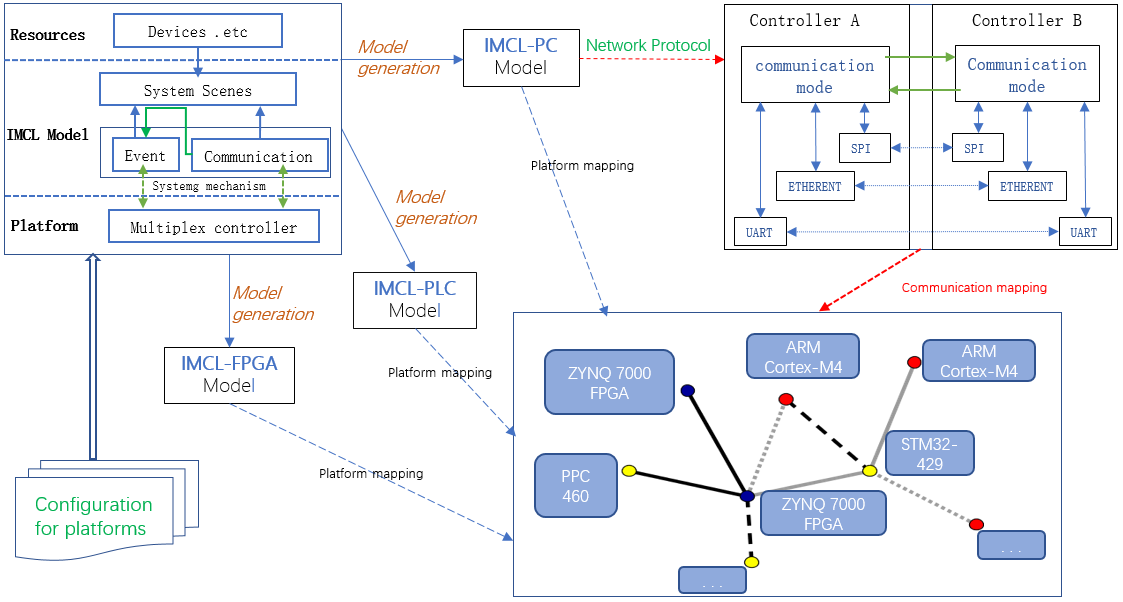
\includegraphics[height=1.4in, width=2.8in]{approach}
  \caption{The approach of IMCL Model to multi-platform code}\label{approach}
\end{figure}

The specific implementation details of the population model generation technique have been proposed in our previous published papers. The advantage of using the ICML modeling method is that we can intelligently split a complex model into multiple sub-models given the constraints of the resource and controller constraints. The sub-models can communicate with each other and achieve the same function as the original model. The generated sub-models correspond to specific target platforms respectively, and the main research work in this paper is to realize the code generation work from the IMCL model to different target platforms.


\subsection{Conversion of IMCL Model and Heterogeneous Platform}
We conduct research on different platforms, including FPGA, PLC, and PC. The research mainly includes how to use IMCL to represent these heterogeneous systems.

\subsubsection{\textbf{Conversion of FPGA and IMCL Model}}
FPGA (Field-Programmable Gate Array, Field Programmable Gate Array), due to its customizable features, is widely used in medical equipment, rail traffic control and other fields. The system developed by the VHDL language used by the FPGA includes the following basic parts:

\begin{itemize}
\item \textbf{Library} \ Declares the repository that the program needs to use, including the std, work, and user-defined libraries. Library contains a variety of design elements, from a program perspective, can be seen as a collection of data.
\item \textbf{Use} \ This section is related to the Library and declares the specific resources used by the corresponding resource library in the Library.
\item \textbf{Entity} \ This area is the entity declaration of the VHDL program and mainly describes the relationship between the input, output, and ports of the system circuit.
\item \textbf{Architecture} \ The architecture is the behavior part of the circuit. The architecture supports the parallel and serial of the program. The main description is its internal implementation process, including data flow, structure description, behavior description and so on.
\item \textbf{Configuration} \ The main purpose of the configuration is to select the required units from the library and form the required system. From the perspective of system resources, it is a process of choice and combination.
\end{itemize}

\begin{figure}[!htb]
  \centering
        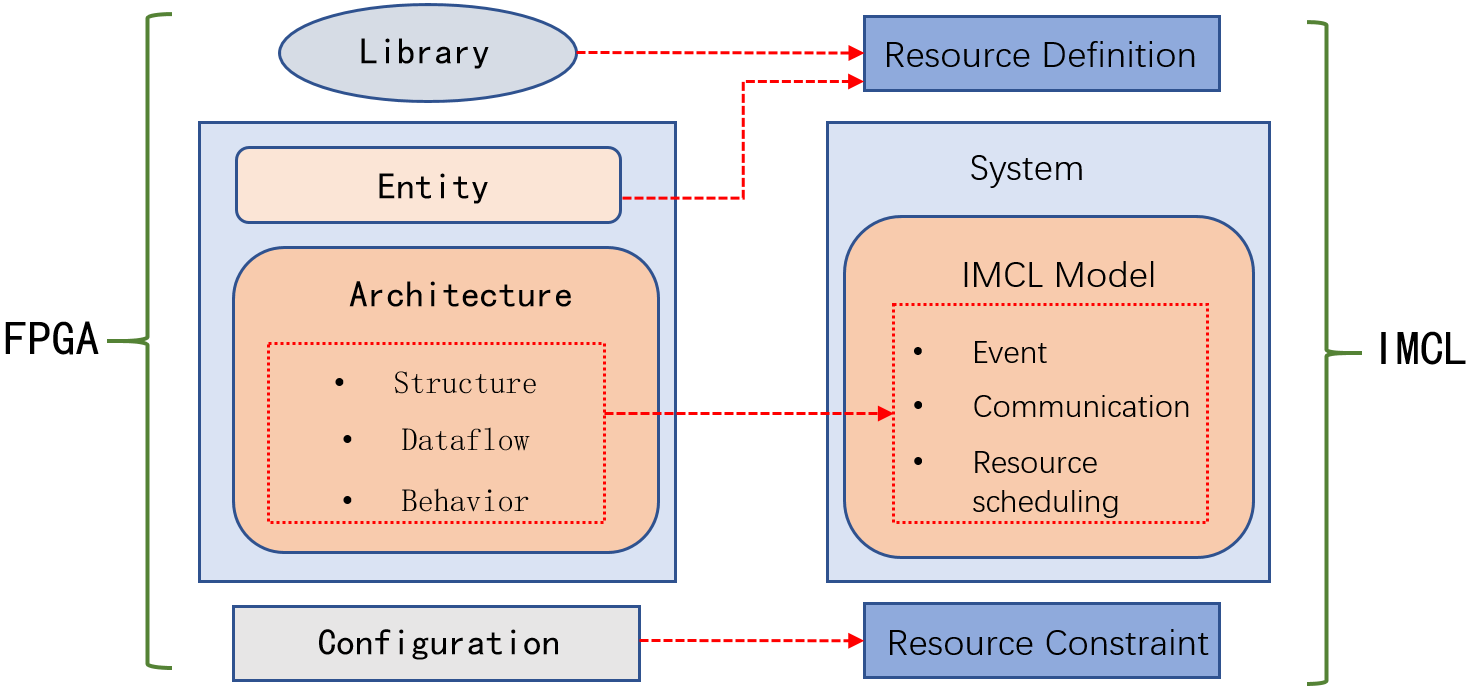
\includegraphics[height=1.4in, width=3.4in]{FPGA2IMCL}
  \caption{The transformation architecture of FPGA and IMCL-Model.}\label{FPGA2IMCL}
\end{figure}

Combined with the characteristics of the previously analyzed IMCL model, we can see that there are commonalities between the two architectures. After ignoring the irrelevant platform details, IMCL can model the behavior described by VHDL. As shown in the figure, the library and package structure represented in VHDL can be abstracted into resources in the process of modeling with IMCL after ignoring platform dependencies. The entity represents the design of the circuit structure of the system and can also be used as a description of resources. The architecture in VHDL mainly includes the structure description, data flow description, and system line description. Essentially, they describe the functional characteristics of the internal structure and correspond to the events described in IMCL.


\subsubsection{\textbf{Conversion of PLC and IMCL Model}}
PLC (Programmable Logic Controller) is a kind of programmable control industrial control computer. PLC takes the microprocessor as the core and realizes the control of the system through software. There are many types of PLCs, but their structural principles are basically the same: they include processors, storage, I/O ports, and network communications. Take the language IEC 61131-3 language by PLC as an example, the design language includes five forms: LD(Ladder Diagram),IL(Instruction List),FBD(Function Block Diagram),SFC(Sequential function chart),ST(Structured Text).

\begin{figure}[!htb]
  \centering
        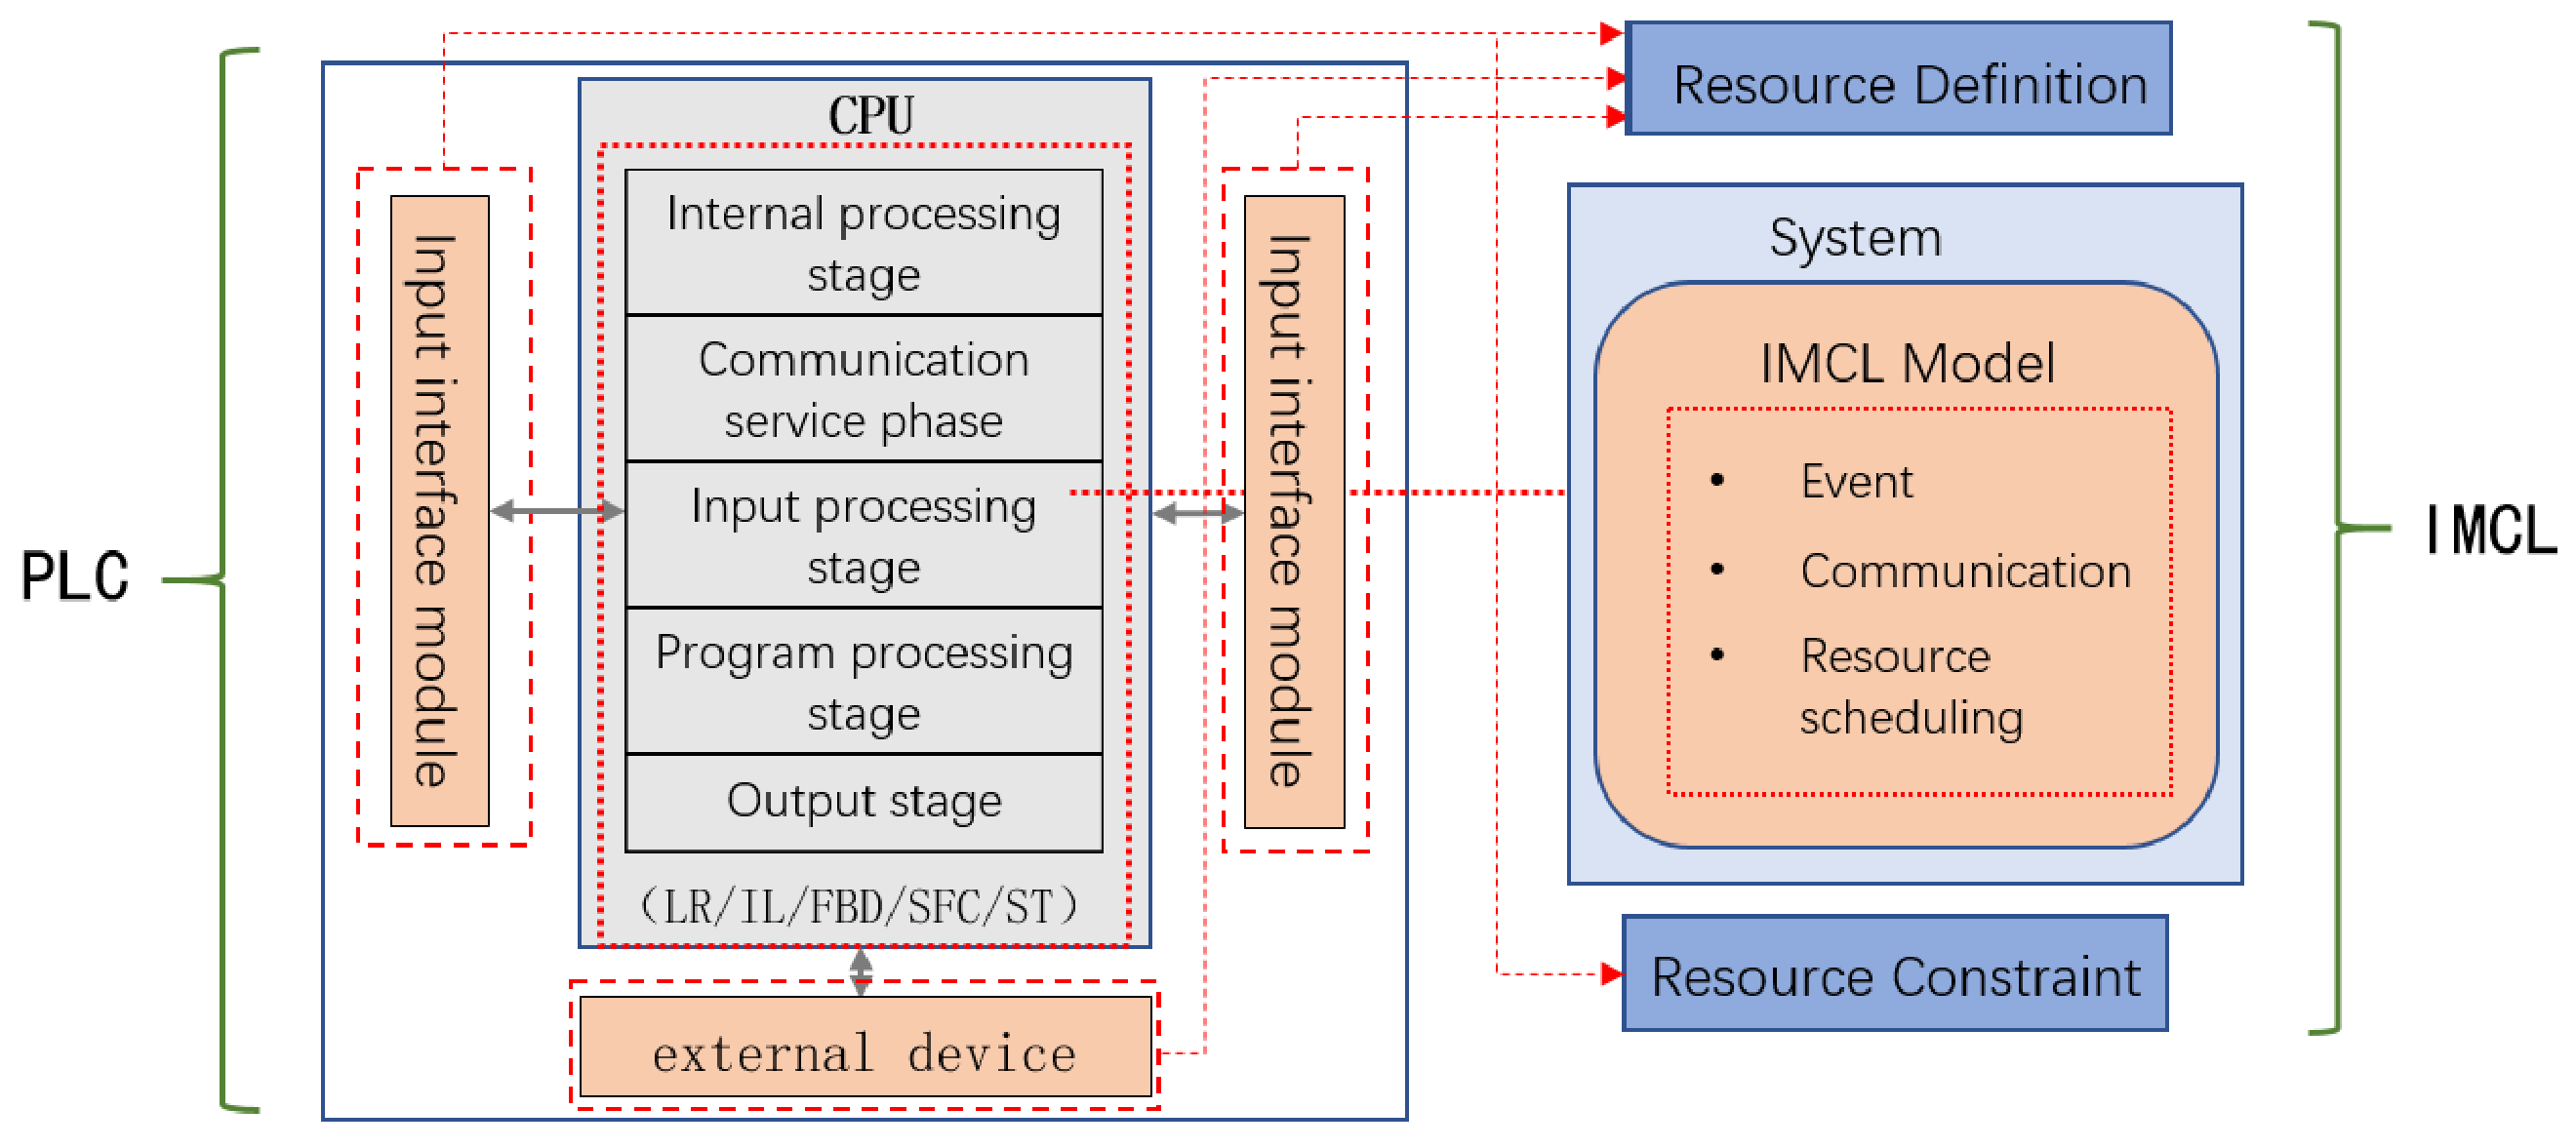
\includegraphics[height=1.4in, width=3.4in]{PLC2IMCL}
  \caption{The transformation architecture of PLC and IMCL-Model.}\label{PLC2IMCL}
\end{figure}

We can use IMCL to represent the operating mode of the PLC. The working phase of the PLC is to periodically scan cyclically, and it will continue to work when there is no interruption or other situations. The general PLC operating mode can be divided into five phases:

\begin{itemize}
  \item \textbf{Internal processing stage}: detecting the system's current ready state and resetting the internal timer;
  \item \textbf{Communication service phase}: The PLC has a communication function. The external control module can communicate with each other and can also receive signal commands from other controllers.
  \item \textbf{Input processing stage}: read the information data of the mounted peripherals and sample the data into the system at one time.
  \item \textbf{Program processing stage}: This stage is the core stage of the PLC control process and is the main body of the PLC program, including condition control, numerical calculation, and logic conversion. This stage reflects the functional behavior of the system.
  \item \textbf{Output stage}: After the main program runs, data is loaded to the outside through the output mechanism.
\end{itemize}

A unified description of the external physical resources associated with the input and output modules, peripherals, etc. The abstract resource object is a program variable, which can facilitate resource scheduling and set constraint conditions. For the main program of the PLC, we extract the main part of the communication services, program execution process, and then use an event-driven way to describe. Finally, the PLC application can be described by the IMCL model.

\subsubsection{Conversion of PC and IMCL Model}
PC (personal computer) is often widely applied to industrial systems because of its advantages such as high-speed processing speed, reliable operation platform, mass storage, networking, and friendly human-computer interaction. For example PCBCS, PC can communicate collaborate with other mainstream PC or PLC systems implement complex functional requirements. In PCBCS, PC's communication technology is one of its greatest advantages. PC can be compatible with almost all communication protocols in the mainstream, so it is very beneficial to the design of complex systems. The common PC system design language is C. Due to its good compatibility, portability, and high execution efficiency, it is widely used in industrial-grade system design.

\begin{figure}[!htb]
  \centering
        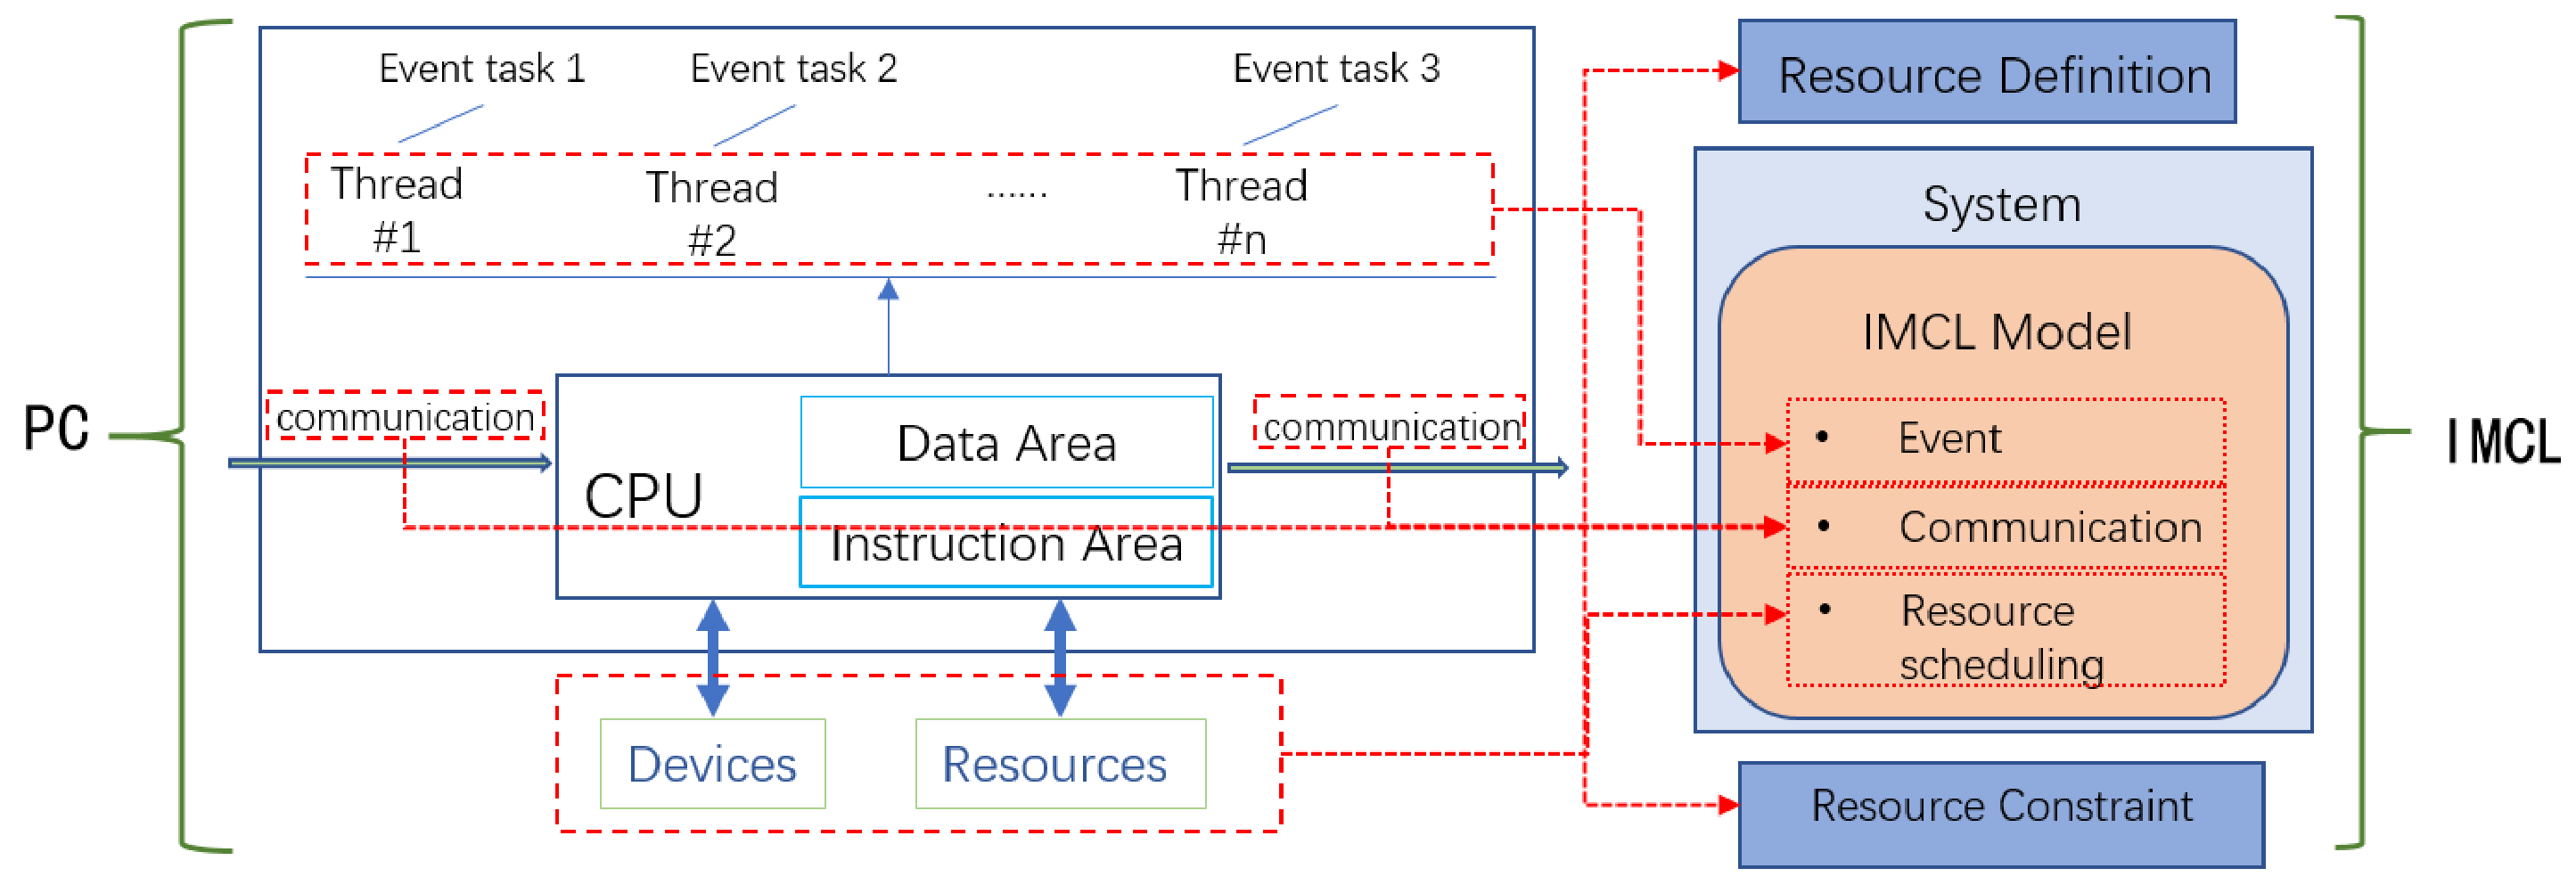
\includegraphics[height=1.4in, width=3.4in]{PC2IMCL}
  \caption{The transformation architecture of PC and IMCL-Model.}\label{PC2IMCL}
\end{figure}

As shown in the figure, a typical PC-style control system design can be represented as shown in the above figure. The CPU is responsible for the execution of the program. The entire system is composed of multiple independent threads. Each thread represents the relevant task. . The system has independent communication, including data input and output. When we use IMCL to model, we represent the multi-threading as a set of concurrent trigger events; the communication of system functions can be represented using the IMCL abstract communication protocol; the control relationship between the system and external device resources, using the resources in IMCL Scheduling to model.


\subsection{Code generation configuration}
The essence of the system model is to abstract away some irrelevant details and only pay attention to a research method to study the characteristics of the object. Therefore, when we want to be able to generate code from model automation, we need to supplement the missing details. In the code generation process from IMCL to a specific target platform, configuration information needed  includes variable conversion, communication protocol method between systems, and the driving relationship between a controller and specific devices. Here we use \emph{Conf} to represent these configuration: $Conf = \langle V_{map}, \ C_{map}, \ D_{map} \rangle$.

$V_{map}$ represents the variable mapping relationship between the model and the specified platform controller: $V_{map} = V_{imcl} \rightarrow (V_{plc} | V_{fpga}| V_{pc})$. The $V_{map}$ refers to the variables $V_{in} \cup V_{out} \cup V_{mess} \cup V_{local} \cup V_{res}$ in IMCL;  $V_{plc} | V_{fpga} | V_{pc}$ corresponds to a collection of variables for specific heterogeneous platforms.

$C_{map}$ represents the mapping relationship between the communication method in the model and the communication protocol used by a particular platform: $C_{map} = C_{imcl} \rightarrow (C_{plc} | C_{fpga} | C_{pc})$. $C_{imcl} = ch!Vmess | ch?V_{mess}$ refers to the formal representation of communications in IMCL; $C_{plc} | C_{fpga} | C_{pc}$ refers to the definition and implementation of specific communication protocols for different platforms.

$D_{map}$ represents the mapping relationship between the driver representation in the model and the drivers of controller and devices in  particular platforms: $D_{map} = D_{imcl} \rightarrow (D_{plc} | D_{fpga} | D_{soc})$.  $D_{imcl}=a_{data} \ll Dev | a_{data} \gg Dev$ refers to the scheduling relationship between the controller and peripheral physical devices in IMCL, and $(D_{plc} | D_{fpga} | D_{pc})$ corresponds to specific target platforms that need to implement the device scheduling driver. 

\section{Rules}
The IMCL model has features such as event triggering, message communication, and resource scheduling. This section describes the conversion rules for converting IMCL models into PLC programs from the perspective of code generation. Common techniques for code generation are based on ASTs, and so are ours. The abstract syntax tree is also called the AST syntax tree, which is the tree structure corresponding to the source code syntax. That is, for source code in a specific programming language, statements in the source code are mapped to each node in the tree by constructing a syntax tree. In the tree structure on the basis of IMCL, given by the code generation rules, the model may be implemented to generate the code for the target platform.


 

\section{Case Study}
An example will be introduced to show how the heterogeneous multi-platform code generation based on IMCL model.


\subsection{The IMCL group model}

\begin{figure}[!htb]
  \centering
        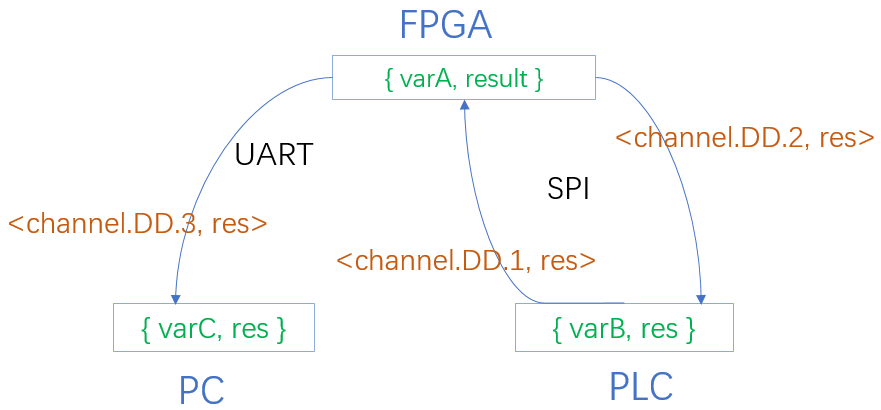
\includegraphics[height=1.5in, width=3.0in]{Compute_example}
  \caption{Heterogeneous computing systems of FPGA, PLC and PC}\label{Compute_example}
\end{figure}
The Fig \ref{Compute_example} is a computing system composed of three different platforms. Each of the three platforms, FPGA, PLC and PC, has its own independent computing and system control functions. Among them use SPI agreement between FPGA and PC, use UART agreement between FPGA and PLC. Each platform's program contains a set of specific variables, and they work together to achieve the ultimate computational task.

\begin{figure}[!tb]
  \centering
        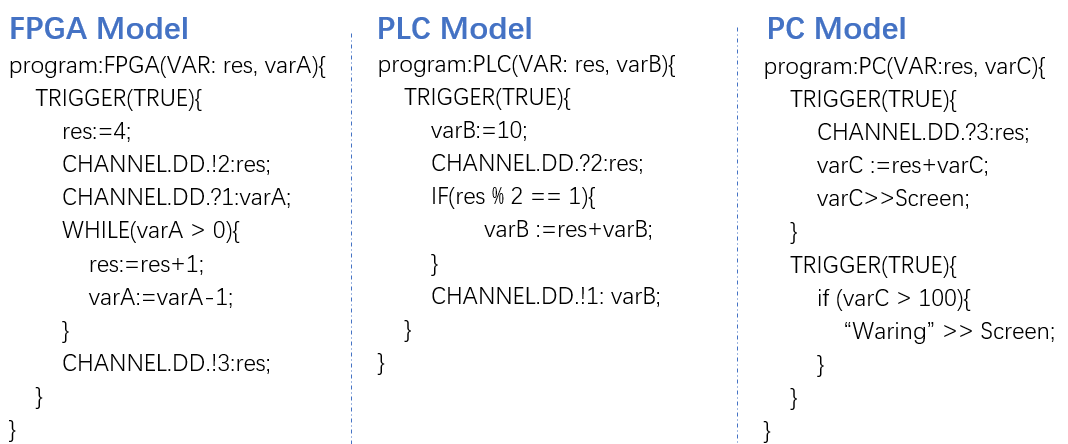
\includegraphics[height=1.8in, width=3.3in]{IMCL_group_models}
  \caption{IMCL group models of FPGA, PLC and PC}\label{group_models}
\end{figure}

\begin{figure}[!thb]
  \centering
        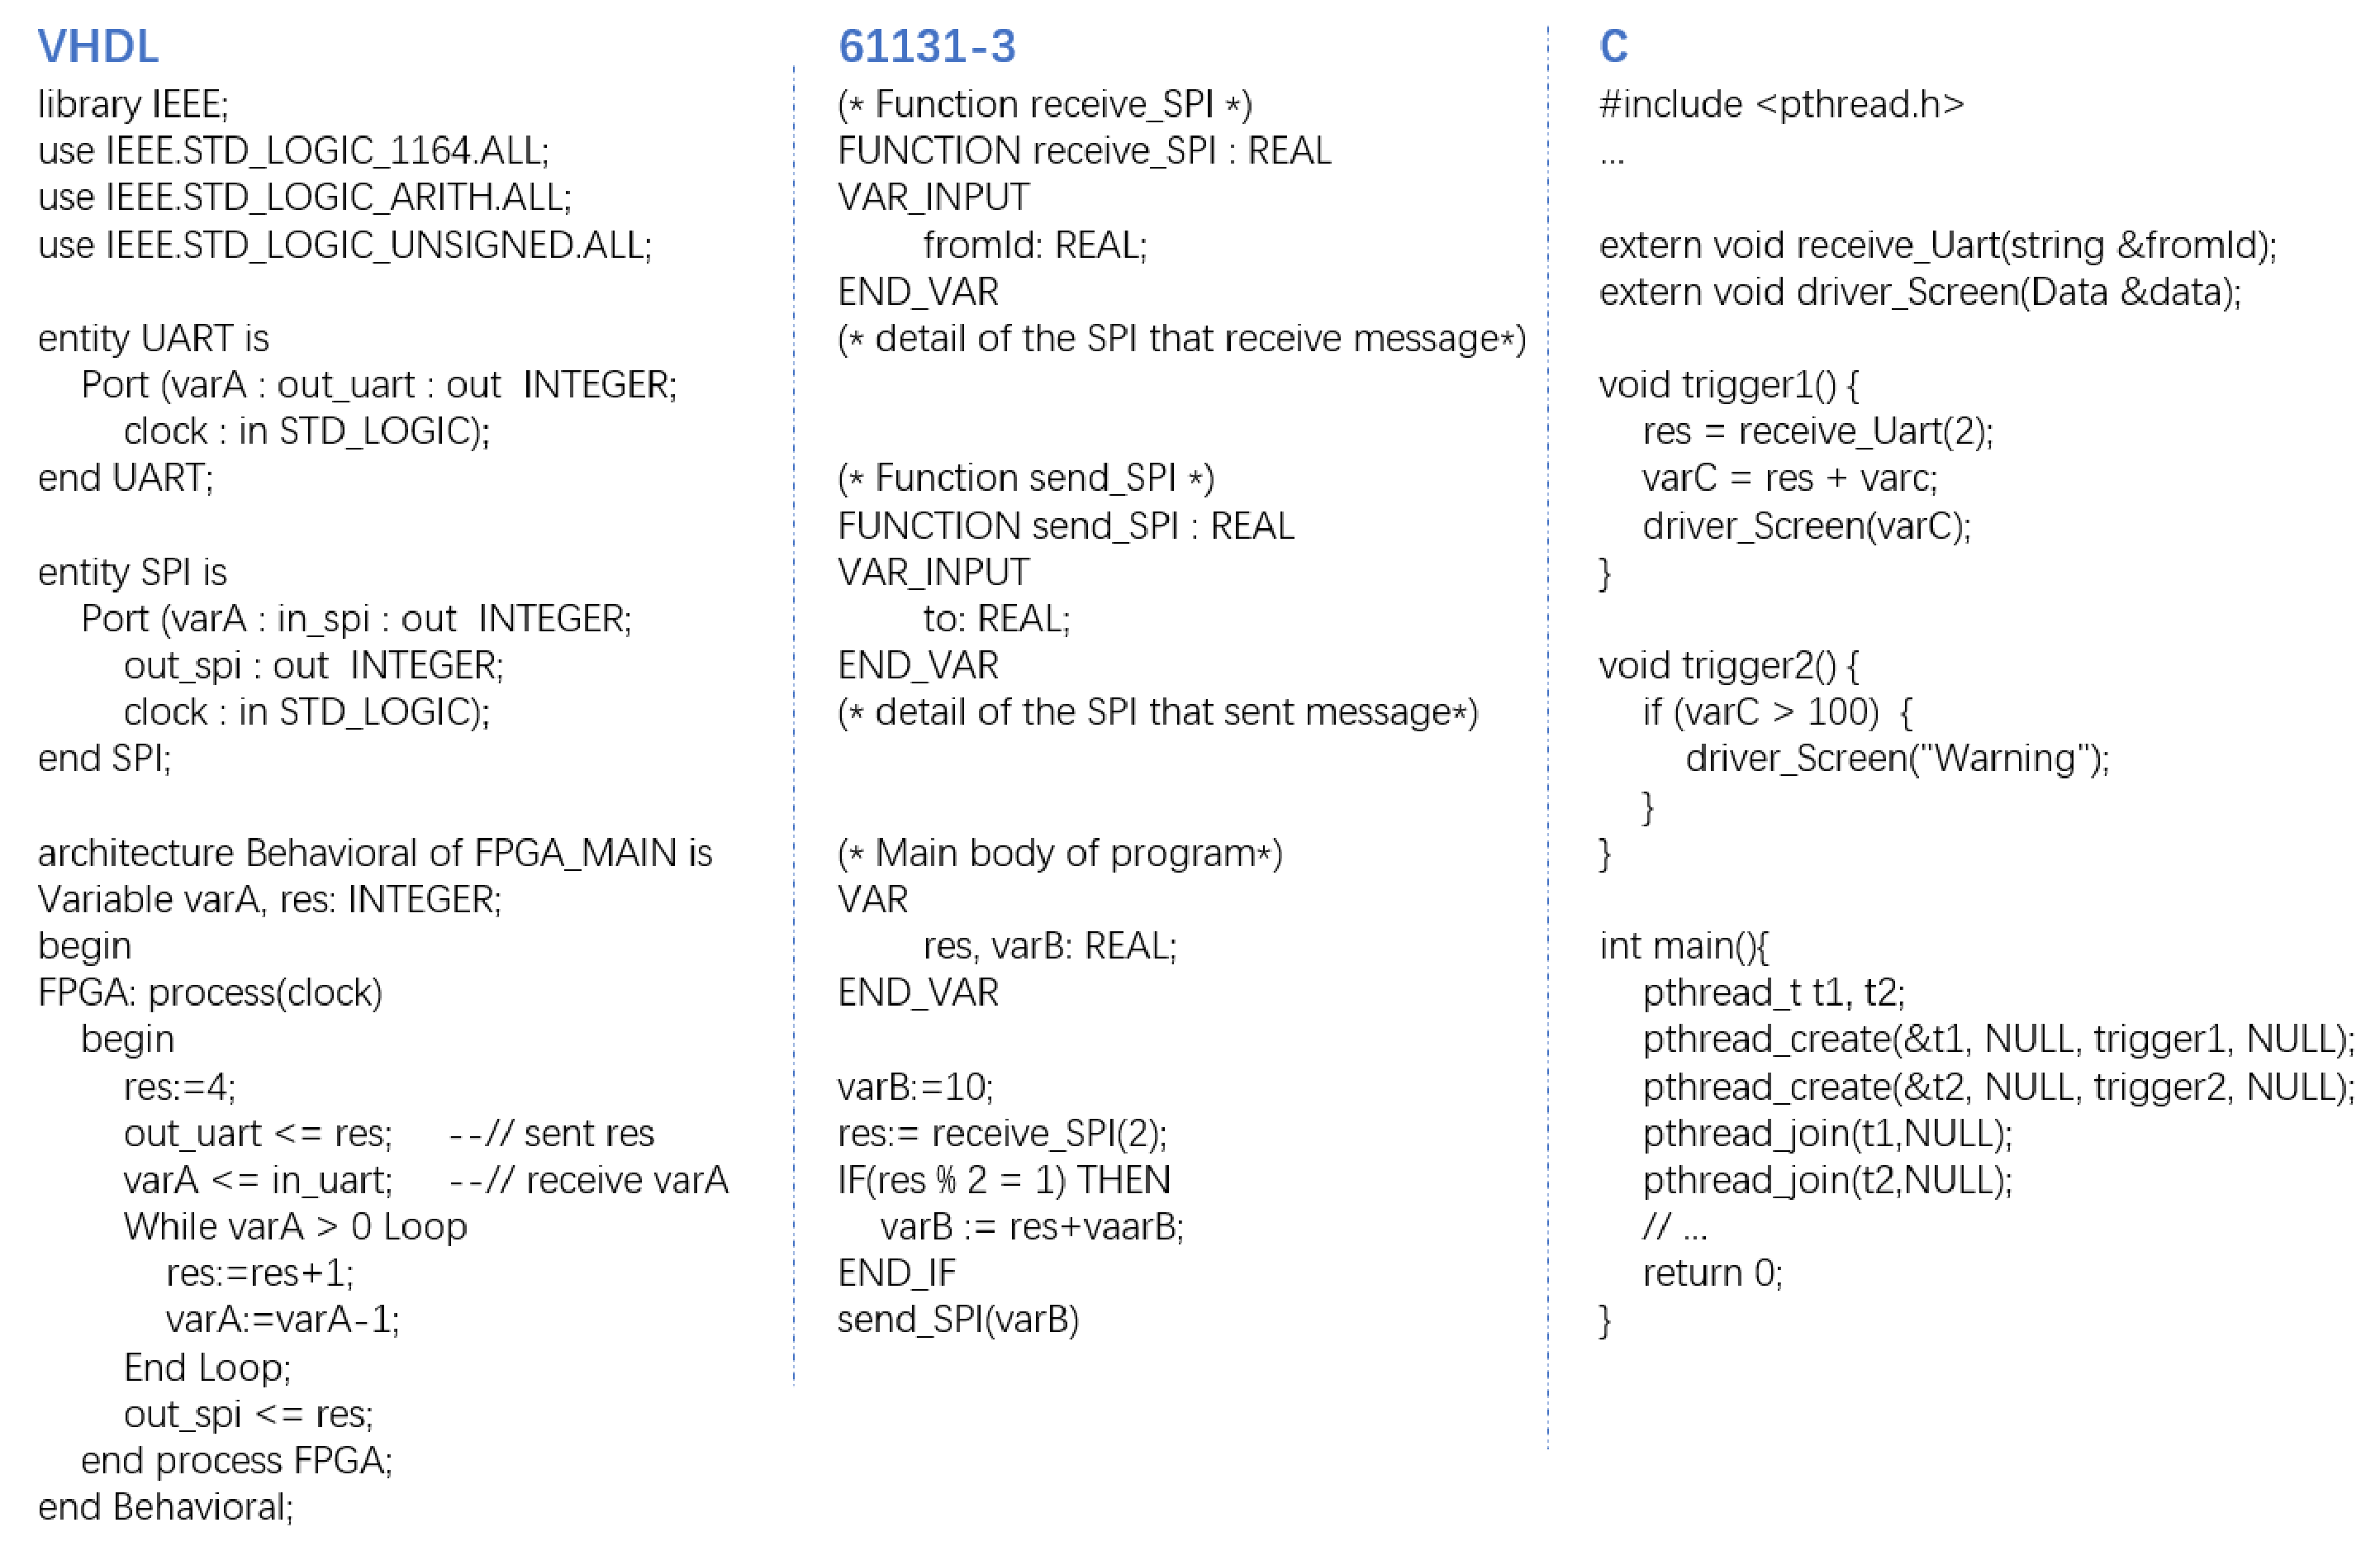
\includegraphics[height=2.0in, width=3.2in]{MultiPlatform_codes_generation}
  \caption{Heterogeneous Multi-platform Code Generation based on IMCL group models(VHDL, 61131-3 and C language)}\label{MultiPlatform_codes_generation}
\end{figure}


Firstly, we use IMCL to describe the entire system. The system model includes three IMCL models that correspond to FPGAs, PCs, and PLCs. Each model contains control functions such as logic operations and communications. The three models communicate data through communications to perform collaborative calculations. The entire system's IMCL model is shown in Fig \ref{group_models}.


\subsection{Multi-platform Code Generation based}


The above three platforms: FPGA, PLC, PC constitute a heterogeneous system. According to the defined five kinds of transformation rules, by analyzing the abstract syntax tree of the IMCL model program, the IMCL group model can finally generate the target platform code corresponding to the corresponding system.

The code in Fig \ref{MultiPlatform_codes_generation} shows the Heterogeneous Multi-platform Code generated by the defined approach. In the VHDL language, we use two Entity to define the communication protocol UART and SPI respectively, and use Behavior to define the function of the main body. In 61131-3, we define the communication function SPI through the functions receive\_SPI and send\_SPI, and use ST language to describe the system's function. In the C language, we implement the communication function by defining the receive\_Uart interface, and define the information scheduling relationship to the device Screen by defining the function driver\_Screen. Based on the analysis of the equivalence relationship between the three platforms and IMCL's system descriptions, we can conclude that our approach to approach code generation is feasible and has application value.
In future work, we will continue to study more efficient conversion methods, and we will explore the conversion rules between IMCL and more platforms. 

\section{Conclusion}
Model-driven code generation techniques have been widely used in system design. For heterogeneous systems, due to their multi-platform nature, it is often difficult to design a system using a single model-driven approach. Therefore, we propose a code generation method that can be used from a single model language to a variety of different target platforms. In this paper, we introduce IMCL features and modeling methods. We have given an approach to converting code from IMCL to the corresponding platform. In this article, we introduce the functional equivalence between the IMCL model and FPGA, PLC, and PC systems. Focused, we have given the rules for conversion between languages. On this basis, by analyzing the syntax tree of the IMCL model, under the given target language conversion rules, we can generate the framework code of the three types of platforms. Our research can improve the flexibility and practicality of model development, allowing developers to put time and energy into the logical design of the system and improve the efficiency of developers. 




% conference papers do not normally have an appendix


% use section* for acknowledgment
\section*{Acknowledgment}
The authors would like to thank...\\
The authors would like to thank...\\
The authors would like to thank...\\
The authors would like to thank...\\
The authors would like to thank...\\
The authors would like to thank...\\


%IEEEhowto:kopka\begin{thebibliography}{1}

\bibitem{IEEEhowto:kopka}
H.~Kopka and P.~W. Daly, \emph{A Guide to \LaTeX}, 3rd~ed.\hskip 1em plus 0.5em minus 0.4em\relax Harlow, England: Addison-Wesley, 1999.

\end{thebibliography}


\bibliographystyle{IEEEtran}
\bibliography{citation}


% that's all folks
\end{document}


